% Sections 7 to 9.

\section{Ember: Human Identity, One Person One Voice}\label{sec:ember}

The whole identity layer rests on a distinction the web of 2026 no longer
knows how to make: who is a person, and who is a program. The dominant
answers measure the body, the iris, or biometry woven into consensus, and
each commits the same founding error: turning a body measurement into a
global identifier and fabricating a perfect target registry for the next
leak. Once the template is engraved somewhere, there is no second chance.
The Ember does not approach the body: it approaches sociability, presence
and time, three things a bot can simulate for a moment but cannot sustain
for years, in view of a community with memory.

The admission of an Ember combines three locks. Presence: a light and
dedicated proof of work, a few seconds of honest computation, signed by
the identity key at each era; it proves a dedicated living machine, not a
phantom identity. The web: each established Ember can sponsor at most two
new Embers per year, and stakes its own Kleos on that sponsorship; a bad
sponsorship costs the sponsor years of reputation, and sponsorship becomes
a rare, expensive and consequence-laden social credit. Time: continuous
incident-free seniority counts in the Tenure layer of Kleos, and tenure
is not manufactured in series. Can a botnet infiltrate? It must first
find established sponsors ready to burn their reputation, at two slots
per year each: the attack becomes more expensive than its value.

\begin{table}[htbp]
\centering
\small
\caption{Biometric personhood versus social personhood.}
\label{tab:personhood}
\begin{tabularx}{\textwidth}{@{}L{3.2cm}YYY@{}}
\toprule
System & Proof used & What is collected & Structural defect \\
\midrule
Worldcoin / World ID & iris scan by the Orb & a biometric template at enrollment & global body registry; single leak target \\
Humanode & biometry woven into consensus & biometric data, even zero-knowledge & the whole chain depends on a body secret \\
Ember (ANTUMBRA) & presence, capped sponsorship, tenure & nothing; no personal data, ever & slow admission; high social cost, assumed \\
\bottomrule
\end{tabularx}
\end{table}

The price of honesty must be named: the Ember is slow to obtain, and that
is a choice. An identity bought by scanning an eye is worth a scan; an
identity that requires a year of community and a sponsor who answers for
you is worth a reputation. The instant governance of the centralized web
has proven what mass without memory is worth: armies of fake accounts.
The governance of ANTUMBRA, one Ember one voice for budgets and identity
rules, will count only voices that cost someone something. That is the
one-computer-one-vote principle carried by NERVA, extended by one storey:
the computer votes for mining, the Ember votes for the community.

\section{Cipher: Accountable Agents by Construction}\label{sec:cipher}

Agent identities are not failed Embers: they are new legal objects,
designed as such. A Cipher registers with three bindings. A sponsor, an
Ember who answers for it: the human at the end of the responsibility
chain, the one who can be summoned. A spending perimeter, a declarative
script verified at every transaction: daily ceiling, list of authorized
recipients, usage markers, validity window. A switch: the sponsor can
revoke the agent in one transaction, and the revocation propagates the
freeze of its spending instantly. An agent's wallet is not a bottomless
private key: it is a bounded mandate, executable by a machine, revocable
by a human, auditable by an accountant.

That structure answers what the agent rails of 2026 do not provide.
Machine-to-machine payment protocols transport stablecoins over HTTP;
the transport layer is excellent. But who pays? In whose name? Up to how
much? Who reimburses if the agent derails? On those questions the current
rails answer with silence, or worse with total transparency that exposes
the agent's budget to every predator on the network. The Cipher brings
the four answers: a verifiable identity, a designated principal,
executable bounds, immediate revocation. An agent of those rails can
moreover be paid through ANTUMBRA: the two layers are complementary, the
rail transports, the trust network qualifies.

\begin{table}[htbp]
\centering
\small
\caption{The transport rail versus the trust layer.}
\label{tab:agents}
\begin{tabularx}{\textwidth}{@{}L{3.8cm}YY@{}}
\toprule
Need of an agent that pays & Current agent rails & ANTUMBRA (Cipher) \\
\midrule
agent identity & transparent address, anonymous & registered identity, with a reputation history \\
accountability & none; the key is the right & designated human sponsor, committed, revocable \\
spending bounds & managed by the agent's code, unverifiable & declarative script executable by the protocol \\
portable reputation & none; every sale restarts at zero & agent Kleos, verifiable by any third party \\
budget privacy & none; everything is public & Veil by default; Lumen for legitimate audit \\
\bottomrule
\end{tabularx}
\end{table}

The founding example, to fix ideas: a small company entrusts an agent
with subscriber invoicing. Its Cipher carries a perimeter, fifty ATU per
day, one authorized recipient per client, an invoicing marker. The
accountant follows everything through a bounded Lumen key; the manager,
sponsor, sees the agent revoked in one transaction if the model drifts;
the agent, on its side, seriously builds its own Kleos, thousands of
settlements without dispute, and that reputation becomes its commercial
asset: future clients will demand an agent with a high Kleos as one
today demands a five-star seller. Trust becomes a career, not a favor.

\section{Kleos: The Reputation Money Cannot Buy}\label{sec:kleos}

Kleos, the glory that only deeds confer, is the heart of the network. It
is a score from 0 to 100, computed by consensus of the signers, therefore
as secure as a balance; non-transferable, therefore unsellable; corroded
by time, therefore demanding real presence; and composed of three layers
whose sum makes trust. The first two are the claimed and corrected
heritage of the two-layer reputation of Axon; the third is the specific
contribution of ANTUMBRA, and the one that locks everything. The overall
formula fits on one line, and each layer has its own rules of rise,
ceiling and corrosion.
\begin{equation}\label{eq:kleos}
\mathrm{Kleos} = \min(100,\; \mathrm{Deed} + \mathrm{Echo} + \mathrm{Tenure}),
\qquad \mathrm{Deed} \le 40,\; \mathrm{Echo} \le 30,\; \mathrm{Tenure} \le 30
\end{equation}

\begin{table}[htbp]
\centering
\small
\caption{Kleos: three layers, three natures of trust.}
\label{tab:kleos}
\begin{tabularx}{\textwidth}{@{}L{3.4cm}L{1.1cm}YYL{2.6cm}@{}}
\toprule
Layer & Cap & What raises it & What lowers it & Can it be bought? \\
\midrule
Deed, observed behavior & 40 & signed checkpoints, dispute-free settlements, service availability, anti-cheat challenges & lost disputes, prolonged silence, fork reports; cheating: reset to zero & no; everything is verified by consensus \\
Echo, peer attestations & 30 & testimonies of plus or minus one, with proof, weighted by the witness's Deed, budget of 0.1 per witness per era & decay of 0.05 per era; mutual detection; anti-spam & with difficulty; capped budget, recent witnesses nearly mute \\
Tenure, continuous seniority & 30 & one point per era of existence without major incident & major incident: definitive collapse of the layer & no; time is not manufactured \\
\bottomrule
\end{tabularx}
\end{table}

Why it cannot be bought, proof by contradiction. An attacker prepared to
spend without limit wants a Kleos of 80 this month. The Deed? They must
actually sign, settle, serve, months of behavior, and every cheat resets
it to zero. The Echo? They must buy witnesses; but the budget of 0.1 per
witness per era caps influence, the weighting by the witness's Deed makes
fresh witnesses nearly mute, and the detection of mutual ratings breaks
symmetric cooperation: they would have to buy established witnesses,
that is, precisely the people with the most to lose. The Tenure? Thirty
points require fifteen years of incident-free existence. Every road leads
to the same wall: the wall of time. In the project that inspired ours,
reputation multiplied capital; here, capital multiplies nothing.
\begin{equation}\label{eq:echo}
\text{Echo budget: } \sum_i |\Delta E_i| \le 0.1 \text{ per witness per era,}
\quad \text{gain per target} \le 2.0 \text{ per era}
\end{equation}

A decisive precision, because it separates this whitepaper from a sales
document: the specification of the social core was submitted to its own
deterministic simulation before being considered settled. Three hundred
lines of code, a fixed seed, sixteen years of history replayed,
invariants verified at every era. The first pass, with the rules of the
second version, did what no re-reading would have done: it showed the
attack succeed. A farm of twenty fake profiles with complicit sponsors,
two sponsorships per year each, impeccable behavior and an unlimited
witness budget, crossed the candidacy threshold at year eight and a
half, before the honest network, and took the fifty-five seats at year
ten. The cause fit in two lines: bought Echo grew four times faster than
organic Echo, and the threshold was crossed without a single year of
tenure.

Four corrective rules, all derived from the thesis of the network, close
that window. R1: candidacy for the Ring requires a Kleos of at least 70
and fifteen eras, seven and a half years, of incident-free existence;
the wall of time also protects finality. R2: a testimony weighs nothing
until the witness has twenty points of Deed; a testimony that counts
comes from someone who has proven something. R3: attestations carry
liability; a target convicted of fraud costs three points of Deed to
each of its witnesses and five to its sponsor: renting one's pen becomes
a slow suicide. R4: the pooled activity of a clique, cross-sales and
mutual ratings, counts at one quarter in the Deed. The second pass, same
maximum attacks, same sixteen years, same seed: zero fake candidates,
zero seats, median Kleos of the fake profiles at 11.9 against 76.5 for
the honest; and the whale with unlimited capital plateaus at 30, never
approaching a seat.

\begin{figure}[htbp]
\centering
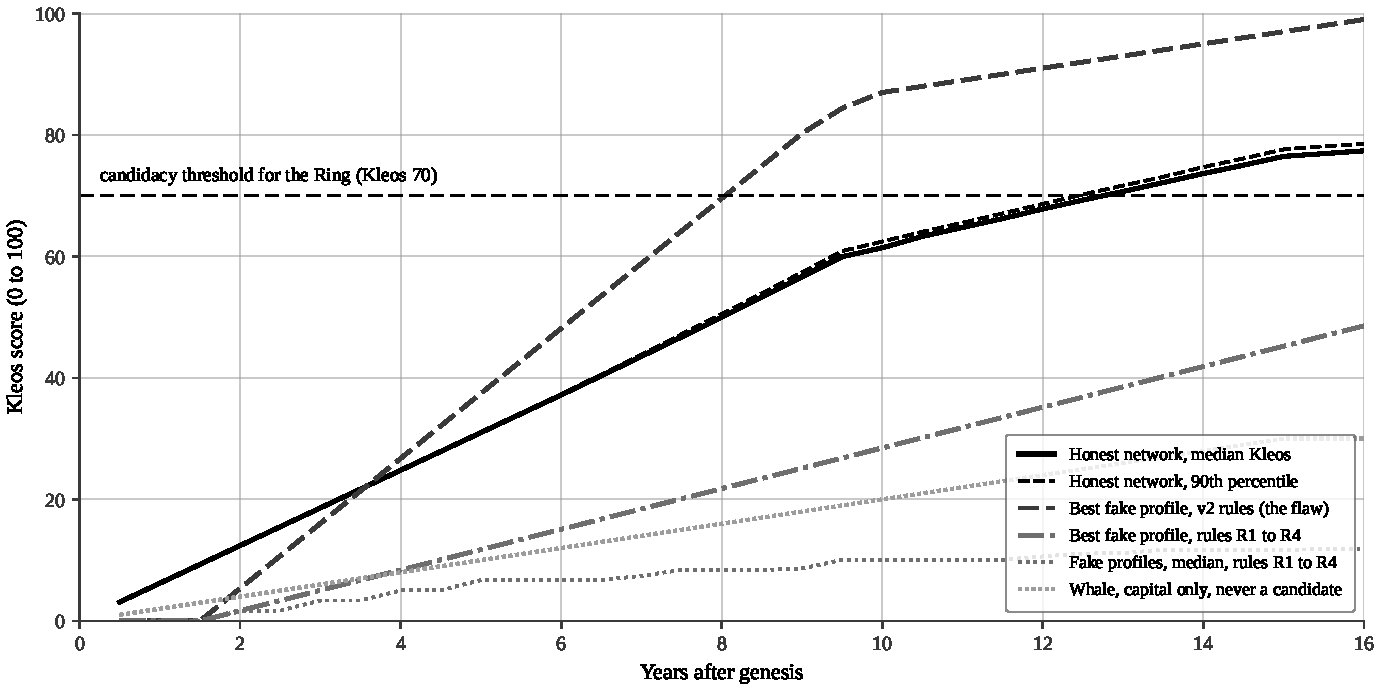
\includegraphics[width=0.94\textwidth]{wp-en-kleos.pdf}
\caption{Kleos trajectories over sixteen years. Under the second-version
rules the best fake profile crosses the candidacy threshold before the
honest network and the attack takes all 55 seats at year 10. Under the
corrective rules R1 to R4 the same maximum attack never approaches the
threshold, and the capital-only whale stays flat at 30. Deterministic
simulation, seed 1618.}
\label{fig:kleos}
\end{figure}

\begin{table}[htbp]
\centering
\small
\caption{Before and after the corrective rules: the same attack, two worlds.}
\label{tab:simres}
\begin{tabularx}{\textwidth}{@{}L{5.6cm}YY@{}}
\toprule
Indicator (16 years, seed 1618) & v2 rules as written & Rules R1 to R4 \\
\midrule
first fake profile candidate & year 8.5, before the honest (12.5) & never \\
worst seats held by the attacker & 55 of 55 (year 10) & 0 of 55 \\
finality control (28 seats) & reached, total capture & never approached \\
median Kleos of fake profiles & about 90 for the oldest & 11.9 (honest: 76.5) \\
whale with unlimited capital & 30.0, never a candidate & 30.0, never a candidate \\
\bottomrule
\end{tabularx}
\end{table}

The simulation thus becomes a regression test: every rule is an expected
number, and every future modification of the protocol will have to pass
the three runs green again. One honest precision to finish: Tenure makes
reputation non-purchasable, but also slow to build; that is a cost, not
only a virtue. Young deserving actors start with an Echo capped by the
weight of their witnesses, and the climb takes eras, not weeks. That
conservatism is assumed: trust is an infrastructure, and infrastructures
are built slowly. Governance may soften it at the margins; it cannot
remove it without breaking the very promise of the network.
